\section{Evolutionary Strategy Composition}\label{sec:evolution}

Genetic programming (GP) has been applied to financial trading for decades, evolving technical rules, portfolio weights, and market-timing strategies \citep{koza1992genetic, poli2008field, lopez2018advances}. Most existing work treats strategies as unstructured program trees, which can produce opaque, overfit solutions that are difficult to interpret or compose. We propose StrategyGenome, a chromosomal representation of trading strategies that encodes domain-specific structure---perception, cognition, execution, risk control, and meta-parameters---in a modular, auditable, and legally interpretable format. This representation enables mutation, crossover, and fitness-based selection tailored to prediction markets.

\subsection{Chromosome Structure}

A \texttt{StrategyGenome} is a Pydantic \texttt{BaseModel} with the following chromosome modules (see Figure~\ref{fig:genome}):

\subsubsection{PerceptionChromosome}

The Perception chromosome defines how the strategy senses the market:
\begin{itemize}
    \item \texttt{data\_sources}: list of data providers (e.g., \texttt{polymarket\_clob}, \texttt{kalshi\_api}, \texttt{coinbase\_klines}).
    \item \texttt{feature\_extractors}: list of feature functions (e.g., \texttt{price\_velocity}, \texttt{orderbook\_imbalance}, \texttt{rsi\_14}, \texttt{vwap}).
    \item \texttt{timeframes}: list of candle intervals (e.g., \texttt{[\"5m\", \"15m\"]}).
    \item \texttt{signal\_aggregation}: method for combining multi-source signals (options: \texttt{weighted\_average}, \texttt{majority\_vote}, \texttt{bayesian\_fusion}).
\end{itemize}

\subsubsection{CognitionChromosome}

The Cognition chromosome encodes the strategy's decision-making logic:
\begin{itemize}
    \item \texttt{entry\_logic}: a trigger type (\texttt{threshold\_cross}, \texttt{pattern\_match}, \texttt{statistical\_arbitrage}, \texttt{event\_driven}, \texttt{momentum\_breakout}) plus a list of \texttt{EntryCondition} objects, each specifying an indicator, operator, value, and weight. Conditions are combined via a conjunction field (\texttt{AND}, \texttt{OR}, or \texttt{weighted\_score}).
    \item \texttt{exit\_logic}: a trigger type (\texttt{time\_based}, \texttt{profit\_target}, \texttt{stop\_loss}, \texttt{trailing\_stop}, \texttt{market\_resolution}, \texttt{spread\_convergence}) plus optional profit and stop-loss percentages and a maximum hold time.
    \item \texttt{market\_selector}: selection criteria (e.g., \texttt{high\_volume}, \texttt{short\_settlement}), a scoring function, and a maximum number of concurrent positions.
\end{itemize}

\subsubsection{ExecutionChromosome}

The Execution chromosome specifies how orders are placed:
\begin{itemize}
    \item \texttt{order\_type}: \texttt{limit}, \texttt{market}, \texttt{fok}, \texttt{ioc}, or \texttt{post\_only}.
    \item \texttt{slippage\_tolerance}: a fraction of the expected price (default 2\%).
    \item \texttt{execution\_speed\_target\_ms}: target latency (default 500 ms).
    \item \texttt{retry\_logic}: how to handle transient failures (\texttt{exponential\_backoff}, \texttt{immediate}, or \texttt{abandon}).
    \item \texttt{atomic\_multi\_leg}: whether multi-leg orders are executed atomically.
\end{itemize}

\subsubsection{RiskChromosome}

The Risk chromosome encodes position-sizing and risk-management parameters that are validated by the \texttt{RiskManager}:
\begin{itemize}
    \item \texttt{position\_sizing\_model}: \texttt{kelly\_fraction}, \texttt{fixed\_fraction}, \texttt{volatility\_targeted}, or \texttt{optimal\_f}.
    \item \texttt{kelly\_fraction}: the fraction of Kelly's optimal bet (default 0.30, bounded between 0.05 and 0.50).
    \item \texttt{max\_position\_fraction}: maximum position size as a fraction of bankroll (default 8\%, bounded between 1\% and 25\%).
    \item \texttt{max\_total\_exposure\_fraction}: total portfolio exposure limit (default 70\%).
    \item \texttt{daily\_drawdown\_limit\_pct} and \texttt{weekly\_drawdown\_limit\_pct}.
    \item \texttt{correlation\_aware\_sizing}: whether to reduce sizes for correlated positions.
\end{itemize}

\subsubsection{MetaChromosome}

The Meta chromosome governs the strategy's self-optimization behavior:
\begin{itemize}
    \item \texttt{self\_optimization\_enabled}: whether the strategy can request parameter tuning.
    \item \texttt{hyperparameter\_tuning\_frequency}: \texttt{every\_trade}, \texttt{hourly}, \texttt{daily}, or \texttt{weekly}.
    \item \texttt{adaptation\_speed}: \texttt{conservative}, \texttt{moderate}, or \texttt{aggressive}.
    \item \texttt{crossover\_eligibility}: whether the genome can participate in crossover breeding.
    \item \texttt{mutation\_rate}: probability of mutation per generation (default 10\%).
\end{itemize}

\subsection{Genetic Operators}

\subsubsection{Mutation}

The \texttt{MutationEngine} applies domain-specific mutations with configurable rates. Perception parameters undergo Gaussian mutation (adding normally distributed noise to feature weights and thresholds). Execution parameters undergo uniform mutation (randomly selecting new order types or retry logic from discrete sets). Cognition entry conditions can be added, removed, or perturbed. Each mutation creates a new genome instance; the original is preserved. Mutations are logged in the \texttt{LineageData} of the offspring, recording the parent genome ID, generation number, and creator type (\texttt{\"mutation\"}).

\subsubsection{Crossover}

The \texttt{CrossoverEngine} performs two-point crossover on the chromosome dictionary. Given two parent genomes, the engine selects two random chromosome keys (e.g., \texttt{perception} and \texttt{risk}) and swaps the corresponding chromosome objects between the parents, producing two offspring. Offspring inherit the best-performing chromosome from each parent, with elitism preserving the highest-fitness genome unmodified in the next generation. Crossover is only permitted when both parents have \texttt{crossover\_eligibility=true} in their Meta chromosome.

\subsubsection{Seeding}

The initial population is generated by \texttt{Seed}, which creates 10 \texttt{DRAFT} genomes with randomized chromosome values. Each seeded genome has a unique archetype and random chromosome configurations, ensuring diversity in the initial population. Seeded genomes are created with \texttt{creator=\"human\"} in their lineage, distinguishing them from evolved offspring.

\subsection{Fitness Function}

Fitness is a composite score combining multiple performance metrics, weighted to reflect prediction-market-specific objectives:
\begin{itemize}
    \item \textbf{Sharpe ratio}: risk-adjusted return (higher is better).
    \item \textbf{Win rate}: fraction of profitable trades (higher is better, but de-emphasized relative to Sharpe to discourage overfitting to small samples).
    \item \textbf{Brier score}: calibration of probability estimates (lower is better; 0.25 is perfectly calibrated for binary outcomes) \citep{brier1950verification}.
    \item \textbf{Maximum drawdown}: worst peak-to-trough decline (lower is better, with a hard penalty above 20\%).
    \item \textbf{Profit factor}: gross profit divided by gross loss (higher is better).
    \item \textbf{Alpha per trade}: average excess return per trade (higher is better).
    \item \textbf{Capital rotation efficiency}: number of trades normalized by bankroll turnover (higher is better).
\end{itemize}

The composite fitness score is a weighted sum, with Brier score receiving elevated weight because well-calibrated probability estimates are essential for profitable prediction-market trading. Fitness scores are cached in \texttt{FitnessMetrics} to avoid recomputation.

\subsection{Lifecycle Integration}

StrategyGenome instances progress through the same stages as regular experiments: \texttt{DRAFT} $\rightarrow$ \texttt{SHADOW} $\rightarrow$ \texttt{PAPER} $\rightarrow$ \texttt{LIVE} $\rightarrow$ \texttt{BREEDING} $\rightarrow$ \texttt{LEGEND} $\rightarrow$ \texttt{GRAVEYARD}. Genomes in \texttt{BREEDING} status are actively crossed with others to produce offspring. Genomes that demonstrate sustained excellence (multiple generations of positive fitness) are promoted to \texttt{LEGEND} status, where they serve as elite donors for future crossover. Genomes that fail health checks receive a \texttt{DeathCertificate} recording the cause of death, final metrics, and whether rehabilitation is possible.

\begin{figure}[H]
    \centering
    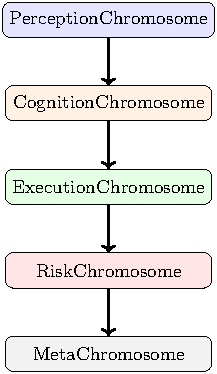
\includegraphics[width=0.95\textwidth]{figures/genome.pdf}
    \caption{StrategyGenome chromosome structure. The Perception chromosome defines data sources and feature extractors; the Cognition chromosome encodes entry logic, exit logic, and market selection criteria; the Execution chromosome specifies order types and execution parameters; the Risk chromosome enforces position sizing and drawdown limits; the Meta chromosome controls self-optimization and mutation rate.}
    \label{fig:genome}
\end{figure}

The StrategyGenome approach is not a claim that genetic programming itself is novel. Rather, our contribution is the domain-specific chromosomal decomposition---the separation of perception, cognition, execution, and risk into modular, interpretable, and composable units---and the tight integration of the genome lifecycle with the bounded autonomy framework described in Section~\ref{sec:autonomy}. This integration ensures that evolved strategies never bypass deterministic risk gates, a combination that, to our knowledge, has not been previously demonstrated in autonomous financial systems.
